% Template for PLoS
% Version 3.1 February 2015
%
% To compile to pdf, run:
% latex plos.template
% bibtex plos.template
% latex plos.template
% latex plos.template
% dvipdf plos.template
%
% % % % % % % % % % % % % % % % % % % % % %
%
% -- IMPORTANT NOTE
%
% This template contains comments intended 
% to minimize problems and delays during our production 
% process. Please follow the template instructions
% whenever possible.
%
% % % % % % % % % % % % % % % % % % % % % % % 
%
% Once your paper is accepted for publication, 
% PLEASE REMOVE ALL TRACKED CHANGES in this file and leave only
% the final text of your manuscript.
%
% There are no restrictions on package use within the LaTeX files except that 
% no packages listed in the template may be deleted.
%
% Please do not include colors or graphics in the text.
%
% Please do not create a heading level below \subsection. For 3rd level headings, use \paragraph{}.
%
% % % % % % % % % % % % % % % % % % % % % % %
%
% -- FIGURES AND TABLES
%
% Please include tables/figure captions directly after the paragraph where they are first cited in the text.
%
% DO NOT INCLUDE GRAPHICS IN YOUR MANUSCRIPT
% - Figures should be uploaded separately from your manuscript file. 
% - Figures generated using LaTeX should be extracted and removed from the PDF before submission. 
% - Figures containing multiple panels/subfigures must be combined into one image file before submission.
% For figure citations, please use "Fig." instead of "Figure".
% See http://www.plosone.org/static/figureGuidelines for PLOS figure guidelines.
%
% Tables should be cell-based and may not contain:
% - tabs/spacing/line breaks within cells to alter layout or alignment
% - vertically-merged cells (no tabular environments within tabular environments, do not use \multirow)
% - colors, shading, or graphic objects
% See http://www.plosone.org/static/figureGuidelines#tables for table guidelines.
%
% For tables that exceed the width of the text column, use the adjustwidth environment as illustrated in the example table in text below.
%
% % % % % % % % % % % % % % % % % % % % % % % %
%
% -- EQUATIONS, MATH SYMBOLS, SUBSCRIPTS, AND SUPERSCRIPTS
%
% IMPORTANT
% Below are a few tips to help format your equations and other special characters according to our specifications. For more tips to help reduce the possibility of formatting errors during conversion, please see our LaTeX guidelines at http://www.plosone.org/static/latexGuidelines
%
% Please be sure to include all portions of an equation in the math environment.
%
% Do not include text that is not math in the math environment. For example, CO2 will be CO\textsubscript{2}.
%
% Please add line breaks to long display equations when possible in order to fit size of the column. 
%
% For inline equations, please do not include punctuation (commas, etc) within the math environment unless this is part of the equation.
%
% % % % % % % % % % % % % % % % % % % % % % % % 
%
% Please contact latex@plos.org with any questions.
%
% % % % % % % % % % % % % % % % % % % % % % % %

\documentclass[10pt,letterpaper]{article}
\usepackage[top=0.85in,left=2.75in,footskip=0.75in]{geometry}

% Use adjustwidth environment to exceed column width (see example table in text)
\usepackage{changepage}

% Use Unicode characters when possible
\usepackage[utf8]{inputenc}

% textcomp package and marvosym package for additional characters
\usepackage{textcomp,marvosym}

% fixltx2e package for \textsubscript
\usepackage{fixltx2e}

% amsmath and amssymb packages, useful for mathematical formulas and symbols
\usepackage{amsmath,amssymb}

% cite package, to clean up citations in the main text. Do not remove.
\usepackage{cite}

% Use nameref to cite supporting information files (see Supporting Information section for more info)
\usepackage{nameref,hyperref}

% line numbers
\usepackage[right]{lineno}

\usepackage{graphicx} 

\usepackage{amssymb}
\usepackage{bm}
% \graphicspath{{./figures/}} % save all figures in the same directory

\newcommand{\given}{\mid}
\newcommand{\me}{\mathrm{e}} % use for base of the natural logarithm
\newcommand{\md}{\mathrm{d}} % use for base of the natural logarithm
\newcommand{\mean}{\mathrm{E}}
\newcommand{\Normal}{\mathcal{N}}
\newcommand{\argmax}{\operatornamewithlimits{argmax}}
\newcommand{\like}{\mathcal{L}}

% ligatures disabled
\usepackage{microtype}
\DisableLigatures[f]{encoding = *, family = * }


\usepackage{bm}
% rotating package for sideways tables
\usepackage{rotating}

% Remove comment for double spacing
%\usepackage{setspace} 
%\doublespacing

% Text layout
\raggedright
\setlength{\parindent}{0.5cm}
\textwidth 5.25in 
\textheight 8.75in

% Bold the 'Figure #' in the caption and separate it from the title/caption with a period
% Captions will be left justified
\usepackage[aboveskip=1pt,labelfont=bf,labelsep=period,justification=raggedright,singlelinecheck=off]{caption}

% Use the PLoS provided BiBTeX style
\bibliographystyle{plos2015}

% Remove brackets from numbering in List of References
\makeatletter
\renewcommand{\@biblabel}[1]{\quad#1.}
\makeatother

% Leave date blank
\date{}

% Header and Footer with logo
\usepackage{lastpage,fancyhdr,graphicx}
\nonstopmode  % to allow pdflatex to compile even if errors are raised (e.g. missing figures)
\usepackage{epstopdf}
\pagestyle{myheadings}
\pagestyle{fancy}
\fancyhf{}
\lhead{
\includegraphics[width=2.0in]{PLOS-submission.eps}}
\rfoot{\thepage/\pageref{LastPage}}
\renewcommand{\footrule}{\hrule height 2pt \vspace{2mm}}
\fancyheadoffset[L]{2.25in}
\fancyfootoffset[L]{2.25in}
\lfoot{\sf PLOS}

%% Include all macros below

\newcommand{\lorem}{{\bf LOREM}}
\newcommand{\ipsum}{{\bf IPSUM}}

%% END MACROS SECTION


\begin{document}
\vspace*{0.35in}

% Title must be 250 characters or less.
% Please capitalize all terms in the title except conjunctions, prepositions, and articles.
\begin{flushleft}
{\Large
\textbf\newline{Matrix Ash}
}
\newline
% Insert author names, affiliations and corresponding author email (do not include titles, positions, or degrees).
\\
Sarah Urbut \textsuperscript{1,2},
Gao Wang {1},
%Name3 Surname\textsuperscript{2,\textcurrency a},
%Name4 Surname\textsuperscript{2,\ddag},
%Name5 Surname\textsuperscript{2,\ddag},
%Name6 Surname\textsuperscript{2},
Matthew Stephens \textsuperscript{1,3,\ddag},
with the GTEX Consortium\textsuperscript{\textpilcrow}
\\
\bigskip
\bf{1} Department of Human Genetics/ University of Chicago, Chicago, IL USA
\\
\bf{2} Pritzker School of Medicine/Growth and Development Training Program/University of Chicago, Chicago, IL USA
\\
\bf{3} Department of Statistics/ University of Chicago, Chicago, IL USA

\\
\bigskip

% Insert additional author notes using the symbols described below. Insert symbol callouts after author names as necessary.
% 
% Remove or comment out the author notes below if they aren't used.
%
% Primary Equal Contribution Note
%\Yinyang These authors contributed equally to this work.

% Additional Equal Contribution Note
% Also use this double-dagger symbol for special authorship notes, such as senior authorship.
\ddag These authors also contributed equally to this work.

% Current address notes
%\textcurrency a Insert current address of first author with an address update
% \textcurrency b Insert current address of second author with an address update
% \textcurrency c Insert current address of third author with an address update

% Deceased author note
%\dag Deceased

% Group/Consortium Author Note
\textpilcrow Membership list can be found in the Acknowledgments section.

% Use the asterisk to denote corresponding authorship and provide email address in note below.
* CorrespondingAuthor@institute.edu

\end{flushleft}
% Please keep the abstract below 300 words
\section*{Abstract}
Lorem ipsum dolor sit amet, consectetur adipiscing elit. Curabitur eget porta erat. Morbi consectetur est vel gravida pretium. Suspendisse ut dui eu ante cursus gravida non sed sem. Nullam sapien tellus, commodo id velit id, eleifend volutpat quam. Phasellus mauris velit, dapibus finibus elementum vel, pulvinar non tellus. Nunc pellentesque pretium diam, quis maximus dolor faucibus id. Nunc convallis sodales ante, ut ullamcorper est egestas vitae. Nam sit amet enim ultrices, ultrices elit pulvinar, volutpat risus.


% Please keep the Author Summary between 150 and 200 words
% Use first person. PLOS ONE authors please skip this step. 
% Author Summary not valid for PLOS ONE submissions.   
\section*{Author Summary}
Variation in gene expression is an important mechanism underlying susceptibility to complex disease.  The simultaneous genome-wide assay of gene expression and genetic variation allows the mapping of the genetic factors that underpin individual differences in quantitative levels of expression (expression QTLs; eQTLs). 
By analyzing these effects across multiple tissues, we exploit the information that the effect of the gene-snp pair in one tissue can provide about its effect in alternative tissues.
Furthermore, quantifying the effect size as opposed to simply calling QTLs present or absent reveal many patterns of sharing of effects among tissues which differ in both sign and magnitude.
We provide a novel framework for estimating effect sizes across multiple subgroups, considering the evidence contained in all subgroups jointly, which provides a powerful and detailed insight into quantitative heterogeneity present in the genome.

%The availability of systematically generated eQTL information could provide immediate insight into a biological basis for disease associations identified through genome-wide association (GWA) studies, and can help to identify networks of genes 
%involved in disease pathogenesis (\cite{nicolae_trait-associated_2010, veyrieras_high-resolution_2008}). However, most studies to date have been conducted in a single immortalized peripheral cell type, and it is unclear to what extent these findings will translate to human disease mapping across more varied cell types. 
%Furthermore, even analyses performed on additional cell types are often performed in a single tissue framework \cite{majewski_study_2011,gilad_revealing_2008} and fail to correlate the effect of genetics across multiple tissue types.  The Genotype Tissue Expression Project, GTEx, Project will provide the data necessary to address this situation: by 2016, the resource is expected to enroll a total of approximately 900 post-mortem donors, with approximately 30 tissues collected from each donor, and the project
%will generate extensive genotype data and RNA-seq data on each individual. However,  available methods are limited in their ability to {\it jointly analyze data on all tissues} to maximize power, while
%simultaneously {\it allowing for both qualitative and quantitative differences among eQTLs} present in each tissue.



\linenumbers

\section*{Introduction}
Variation in gene expression is an important mechanism underlying susceptibility to complex disease.

The simultaneous genome-wide assay of gene expression and genetic variation allows the mapping of the genetic factors that underpin individual differences in quantitative levels of expression (expression QTLs; eQTLs). 
The availability of this information provides immediate insight into a biological basis for disease associations identified through genome-wide association (GWA) studies, and can help to identify networks of genes 
involved in disease pathogenesis (\cite{nicolae_trait-associated_2010, veyrieras_high-resolution_2008}).
Available methods are limited not only in their ability to {\it jointly analyze data on all tissues} to maximize power, but also in simultaneously {\it allowing for both qualitative and quantitative differences among eQTLs} present in each tissue.

Initial approaches to quantify the effect of a particular SNP on gene expression considered only one tissue at a time, and ignored the effect of the SNP on gene expression in other tissues.
This fails to exploit the power of  shared genetic variation in effects on expression - i.e. the information that the effect of the gene-snp pair in one tissue can provide about the effect in another- and limits our understanding of multiple-tissue phenotypes.
Furthermore, even past attempts at quantifying heterogeneity of eQTLs using the data across tissues jointly were limited in both the number of tissues considered, and also the level of heterogeneity considered. Qualitative heterogeneity refers to calling a snp `active' or `inactive' in a given tissue. For example, previous work has referred to the setting in which the gene-snp pair is active in all tissues as `shared' and active in only one as 'tissue-specific'  (\cite{flutre_statistical_2013,wen_bayesian_2014}).
However, a QTL may be`active' in all or many tissues and with varying magnitude or sign; we refer to this as quantitative heterogeneity.
 Indeed, our initial motivation came from our analysis of GTEx pilot data, in which we see evidence that many (50\%) QTLs are shared across all nine tissues. In this context, a QTL is called based on whether it demonstrates significant posterior probability of being active in a particular tissue. Applying our hierarchical model to the dataset from Dimas $\it{et a}l$ $\cite{dimas_common_2009}$ with 3 tissues, we found just 8\% of eQTLs are specific to a single tissue, with an estimated 88\% of eQTLs being common to fibroblasts, LCL cells and T-Cells \cite{flutre_statistical_2013}. Not all eQTLs are shared by all tissues; some tissues may share eQTLs more than others. To allow for this, our previous hierarchical model attempted to infer the extent of such sharing by estimating the proportion of eQTL which were shared in various 'configurations' or patterns of binary activity. 
 However, these binary configurations are still $\textit{ limited in their ability to capture continuous variation}$ in levels of activity among tissues in which the SNP is considered active. 
 In fact, as the number of tissues considered increases, perhaps the more interesting and biologically relevant question becomes one of quantitative heterogeneity - that is, how do the patterns of effect vary across tissues in which the SNP is called 'active'.  
Quantifying the effect sizes of the gene-snp pair across tissues considering the evidence contained in all tissues jointly thus reveals new patterns of activity across tissues, which differ in their relationship in sign and magnitude within and between tissues. Thus effects can be 'shared' but not 'consistent' across tissues. The structure of this paper is as follows: we will describe our approach for modeling and estimating these effect sizes across tissues, 

\subsection{Approach} 
We aim to learning about patterns of sharing across tissues within a SNP and among SNPs, which join to help us better understand the global and snp-specific patterns of effects of genetics on gene expression. 
This allows us to make comparisons among tissues in which the QTL is called active, and among gene-snp pairs with a similar degree of activity in a given tissue. 
Thus as an additional level of combining information, we assume that each eQTL may follow a particular pattern of activity characterized by its effects across tissues. Within these groups, the tissues exhibit characteristic patterns of sharing, which can be captured by considering the covariance structure of the genetic effects among tissues. \insert{figure}This lends itself to a mixture model, in which  we assume all the gene-snp pairs arise from a mixture of a finite number of multivariate normal (MVN) distribution, each characterised by the covariance matrix from which the vector of effects is though to arise. For each of $J$ gene-snp pairs, we observe an R dimensional vector of standardized effect sizes $\bm\hat{b}$ and their standard error and assume that these effects descend from some true effect size $\bm{b}$. 



 \begin{equation}
  \bm{b_{j}} | \bm{\pi},\bf{U} \sim \sum_{k,l} \pi_{k,l} \;{\it N}_R(\bm{0}, \omega_l U_{k})
\end{equation}

Here, the covariance matrix $U_{k}$ captures the particular patterns of sharing - variation in effect sizes within and between tissues
 Choice of Uk determines the direction (relative relationship in effect sizes within and between tissues), while $\omega_{l}$ determines the scale of each pattern - the magnitude of the effect size. Thus we recognize that while two EQTL may obey a similar pattern or shape, the absolute scale may vary. For example, two eQTL may both have strong correlation between tissues 1 and 2 with consistently larger effects in 2, but the absolute size of the effects maweeny vary between SNPs.
 Previous work from our lab considered only the idea that the variance of and covariance between two tissues was the same across tissues thought to contain a QTL in a given pattern, or 'configuration',  and thus failed to incorporate the much richer covariance structure between tissues. As a critical innovation on our previous method $(\cite{flutre_statistical_2013,wen_bayesian_2014})$ these matrices contain distinct diagonal and off-diagonal elements which reflect data-specific patterns of variation within and covariance between subgroups (tissues). This captures the variation in effect sizes within and between subgroups better than restricting effects to simply 'shared' or 'unshared' between subgroups. 
 
  Because we can't know the 'true covariance matrix' for each gene-snp pair, we aim to assemble a list which sufficiently captures the various patterns, and then 'learn' the relative proportions of each pattern of sharing from the data. One can now model each vector of effect sizes $\bm{b}$ each as arising from a mixture that captures all the covariance patterns.



Previous work from our lab considered only the idea that the covariance between two tissues was the same across tissues thought to contain a QTL in a given pattern, or 'configuration',  and thus failed to incorporate the much richer covariance structure between tissues. 

The primary novelty of this approach l is {\it to estimate this multivariate posterior distribution on the effect size in a data-sensitive way} - i.e., using the mixture model to capture information about the covariance structure among subgroups (here, tissues). Thus we might identify a situation in which it is common to have large effects in some tissues and not others, and thus if a gene-snp pair demonstrates a small effect in one of the 'off issues', we might be inclined to conclude that it is indeed a member of this particular class and shrink the small effect in this tissue accordingly. However, if we see the same small effect in a setting in which 'similar tissues' have large effects, we might 'shrink' this effect size less, due to our high prior belief in the SNP's effectiveness garnered from adjacent tissues.This is in contrast to a univariate shrinkage approach, in which all effects of the same size would be 'shrunk' equivalently, due to lack of information garnered from adjacent tissues 



An additional novelty is that in learning something about the effect size in each tissue for a given gene-snp pair, we can make statements about the degree of heterogeneity - that is the proportion of the time we expect a SNP to have effects of different sign. We will be confident in our ability to identify the direction of the effect for A SNP with a large effect and relatvilely high precision, and thus we can use an estimate of the posterior mean in each component and the proportion to quantify the distribution of gene SNP pairs who have effects of opposite direction (or lack convincing evidence of effects in a consistent direction across tissues).




%\section*{Results}
%
%Matrix ASH can be used to assess the effect size across subgroups, allowing the effect in one tissue to powerfully inform our estimate of the effect in the other tissues.
%
%
%Considering a scatterplot of our results against the original summary statistics, the ability of Matrix-Ash to selectively shrink only the smallest effect sizes in a manner consistent with the patterns observe din the larger data set. Suppose we observe two small effects: one in which the effect size observed in other tissues is larger, and one in which the other tissues show similarly small effect sizes. The effect size in which alternative tissues show larger effects will not be shrunk to the same degree in which alternative tissues show small effects. because larger effects in alternative tissues lead us to believe that the  SNP belongs to a group or class in which effects are consistently bigger, and if this group is well represented in the data, we will augment the ultimate effect size because there will be a high prior weight on this componenet.
% \begin{figure}[h]
%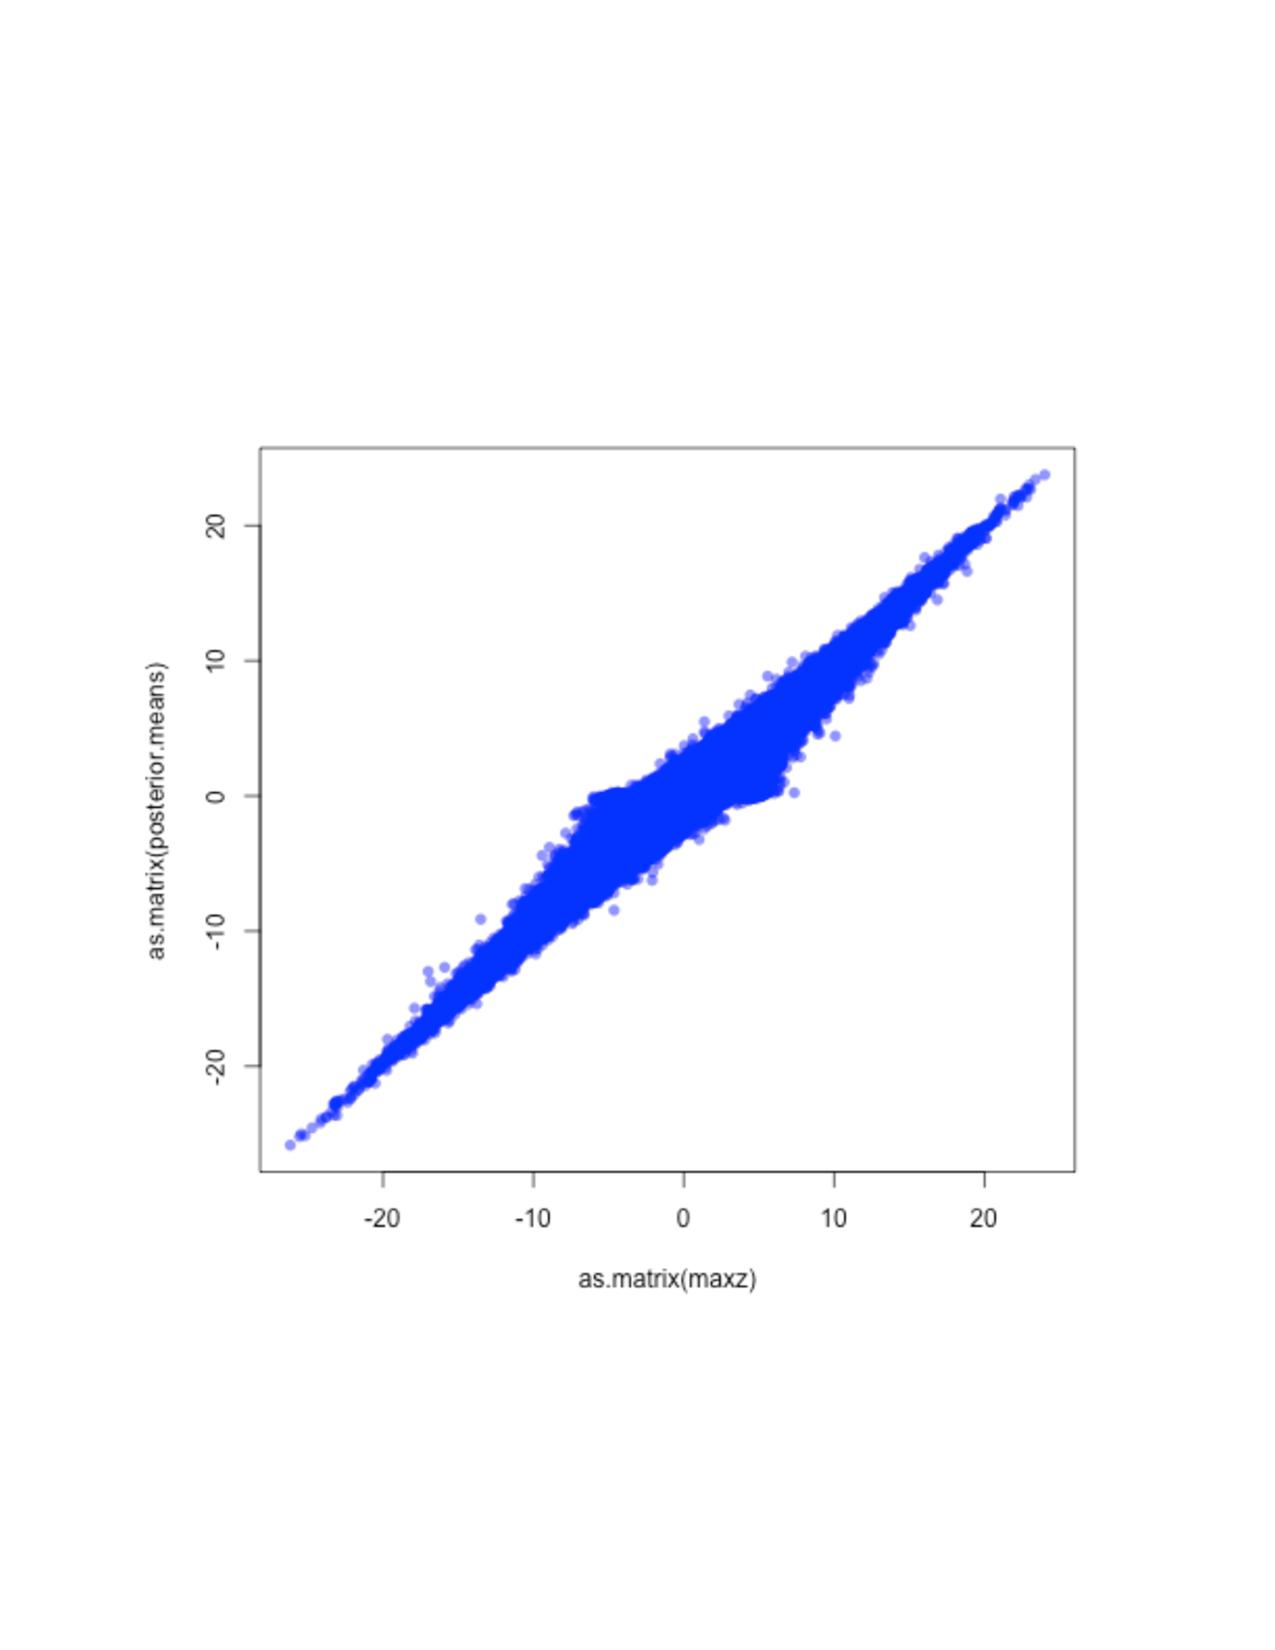
\includegraphics[width=5cm]{scatterplot}
%\caption{Different Shrinkage}
%\end{figure}
%
% \begin{figure}[h]
%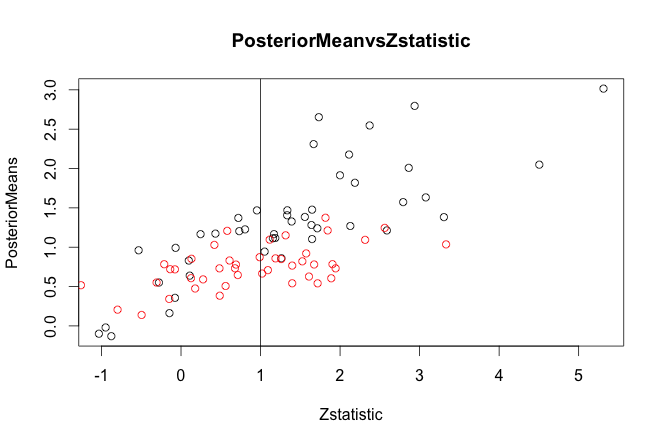
\includegraphics[width=5cm]{selective_shirnk.png}
%\caption{An example in which consistency across tissues shrinks posteriors differently}
%\end{figure}
%
%
%
% \begin{figure}
%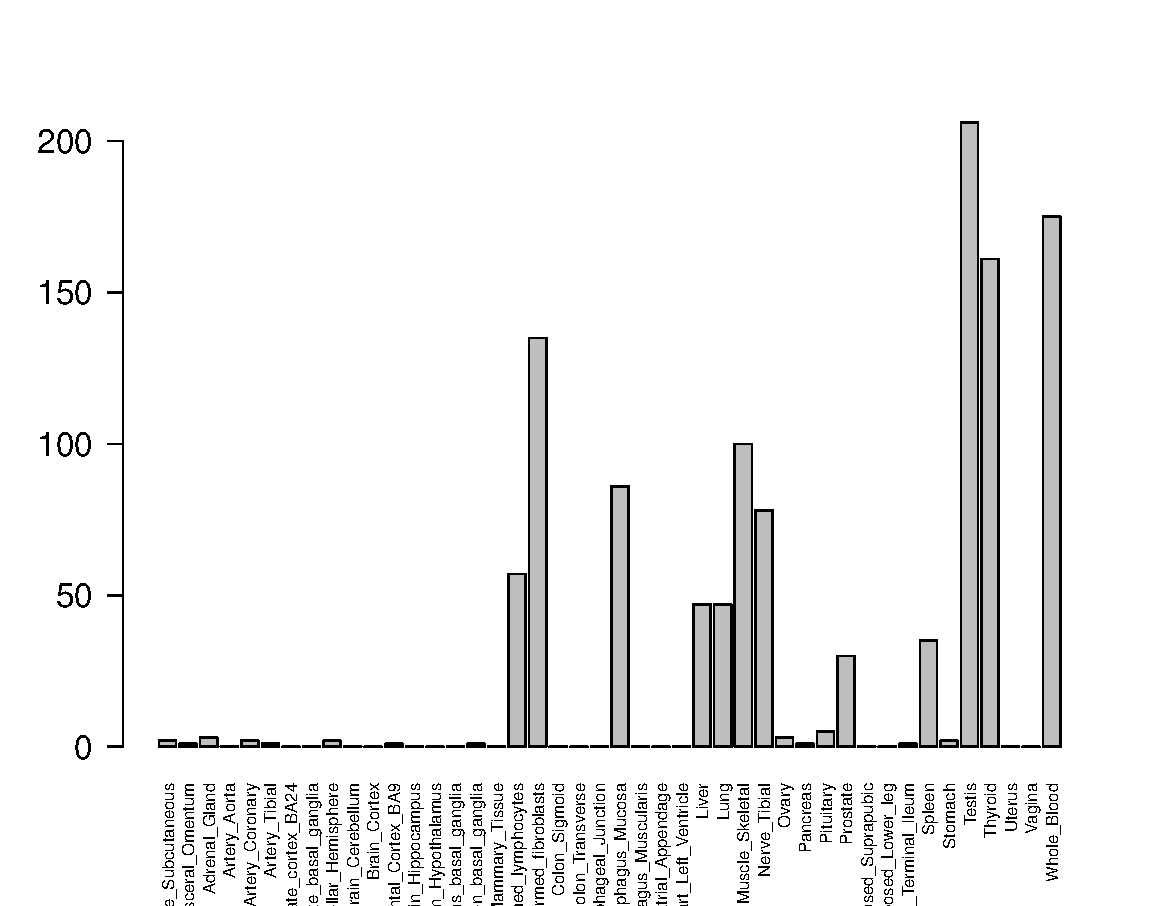
\includegraphics[width=5cm]{TissueSpecific}
%\caption{Tissue Specific Effects}
%\end{figure}
%
%
% \begin{figure}
%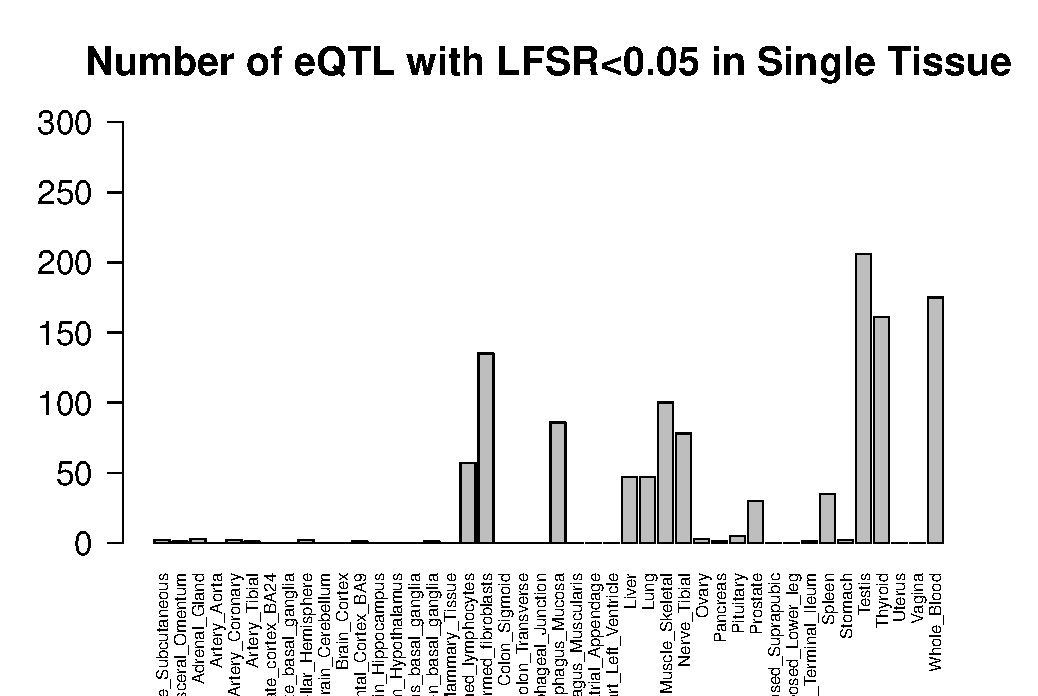
\includegraphics[width=5cm]{lfsr>0.05}
%\caption{An example in which consistency across tissues shrinks posteriors differently}
%\end{figure}
%
%
% \begin{figure}
%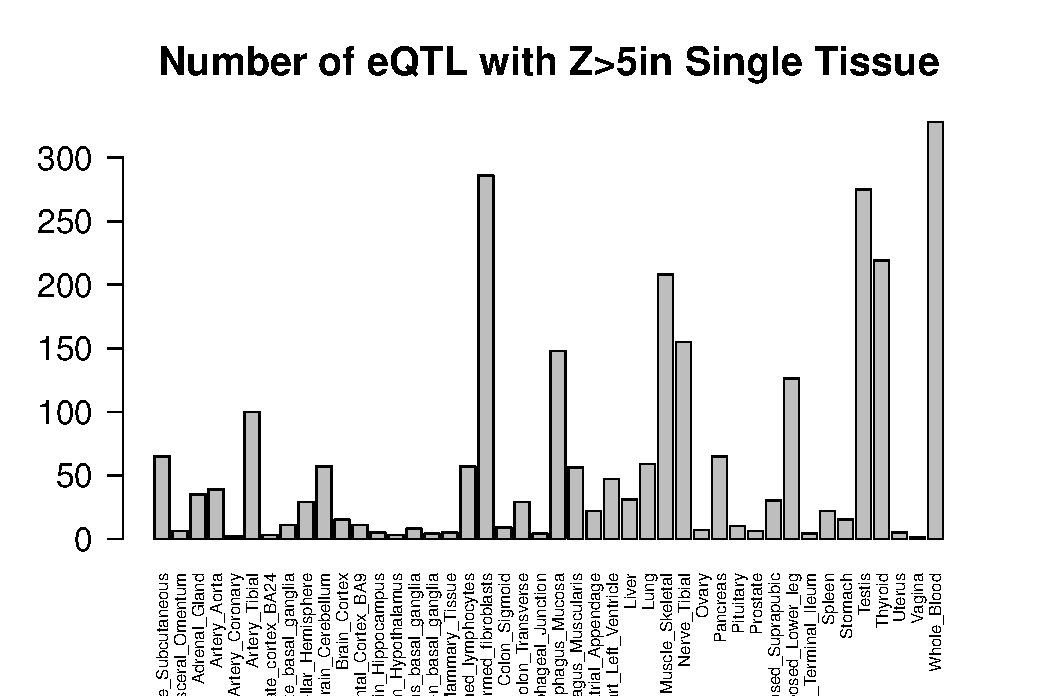
\includegraphics[width=5cm]{z>5}
%\caption{An example in which consistency across tissues shrinks posteriors differently}
%\end{figure}
% \begin{figure}
%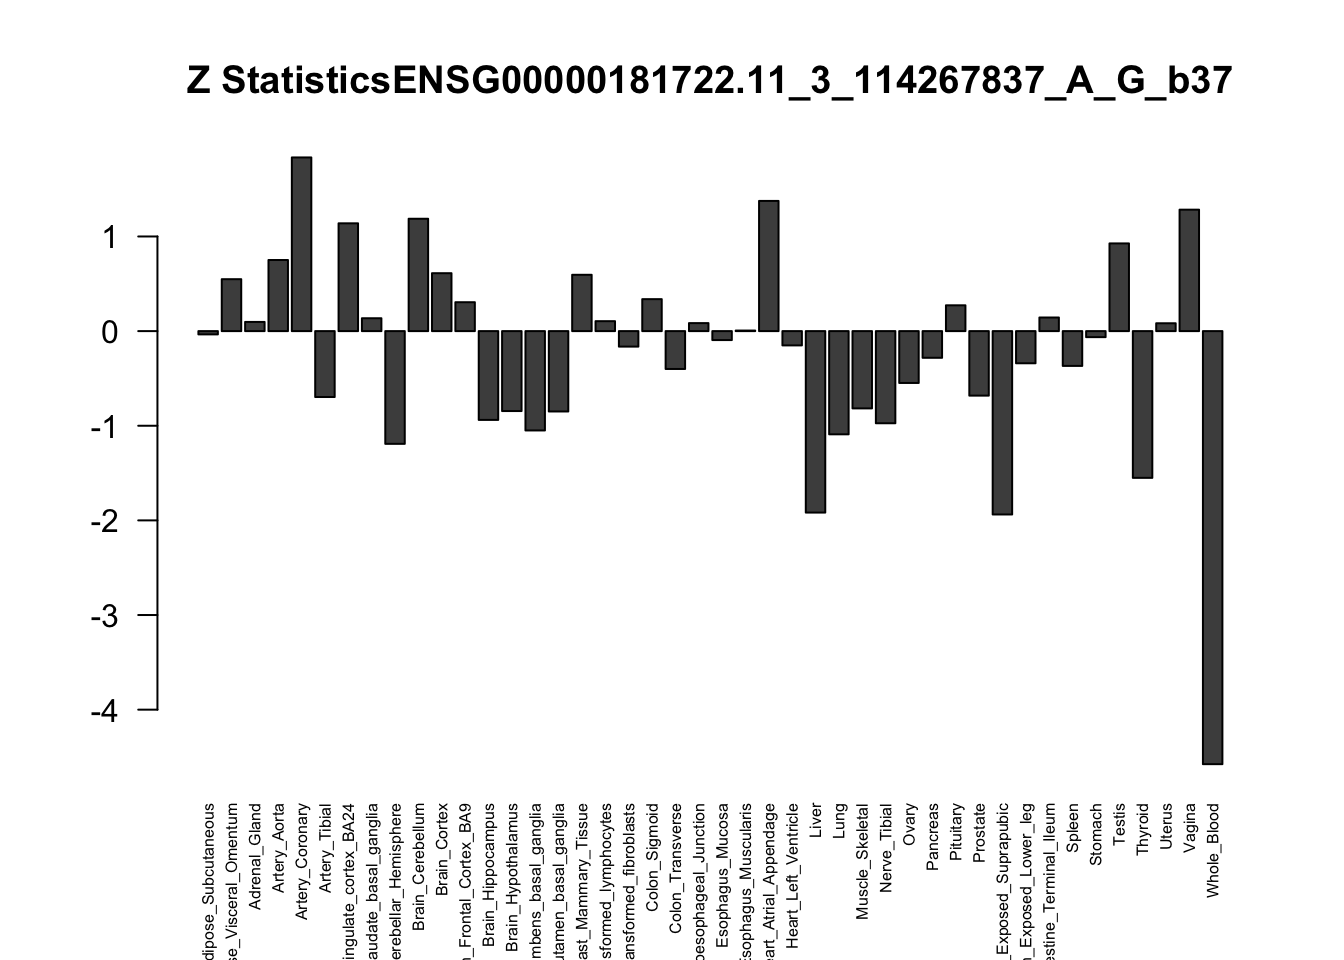
\includegraphics[width=5cm]{singletonz.png}
%\caption{An example in which consistency across tissues shrinks posteriors differently}
%\end{figure}
%
% \begin{figure}
%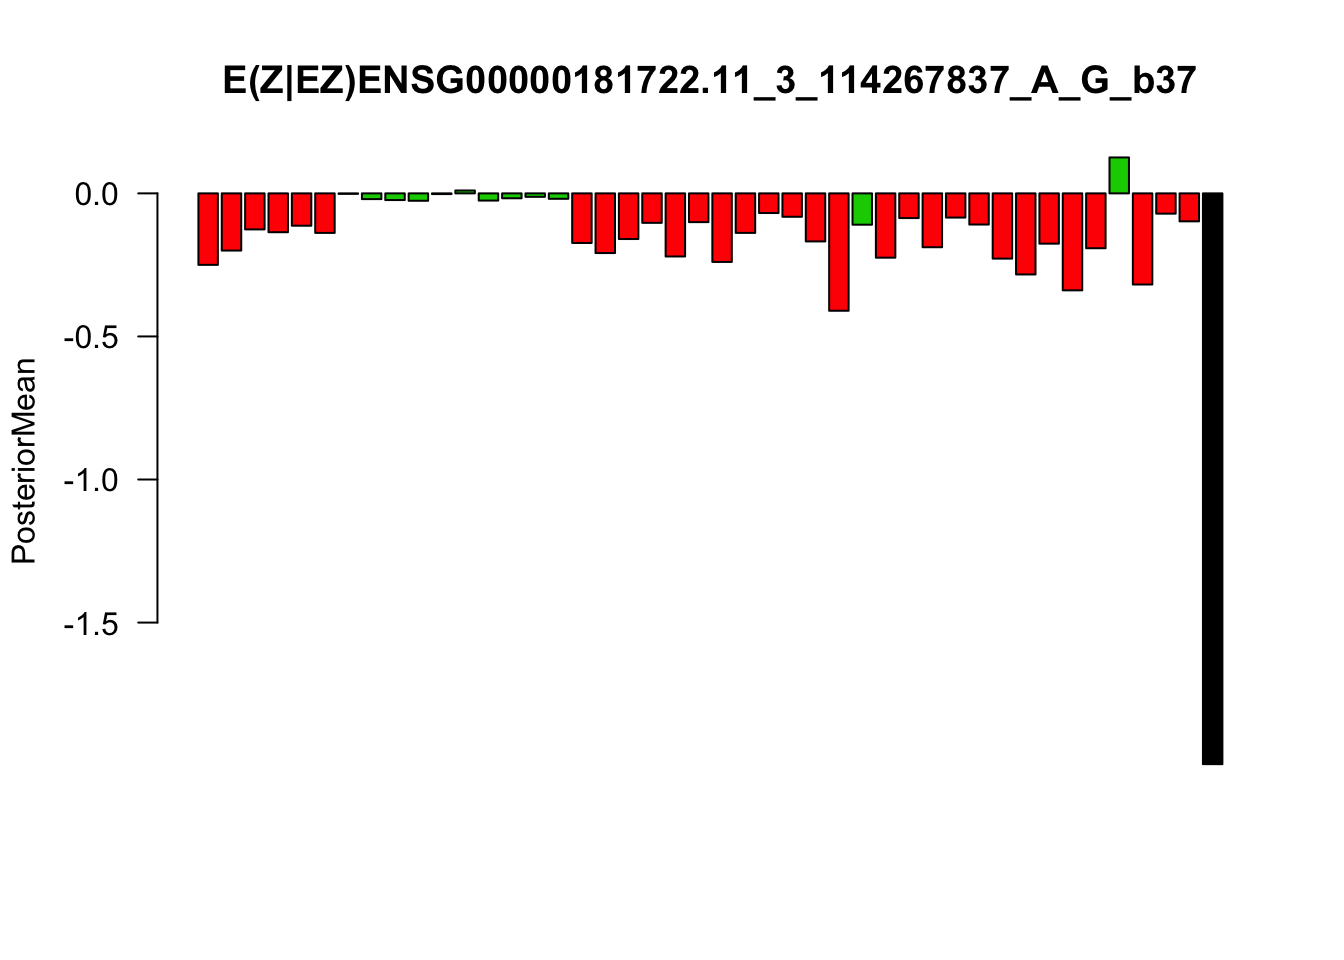
\includegraphics[width=5cm]{singleton.png}
%\caption{An example in which consistency across tissues shrinks posteriors differently}
%\end{figure}
%
% \begin{figure}
%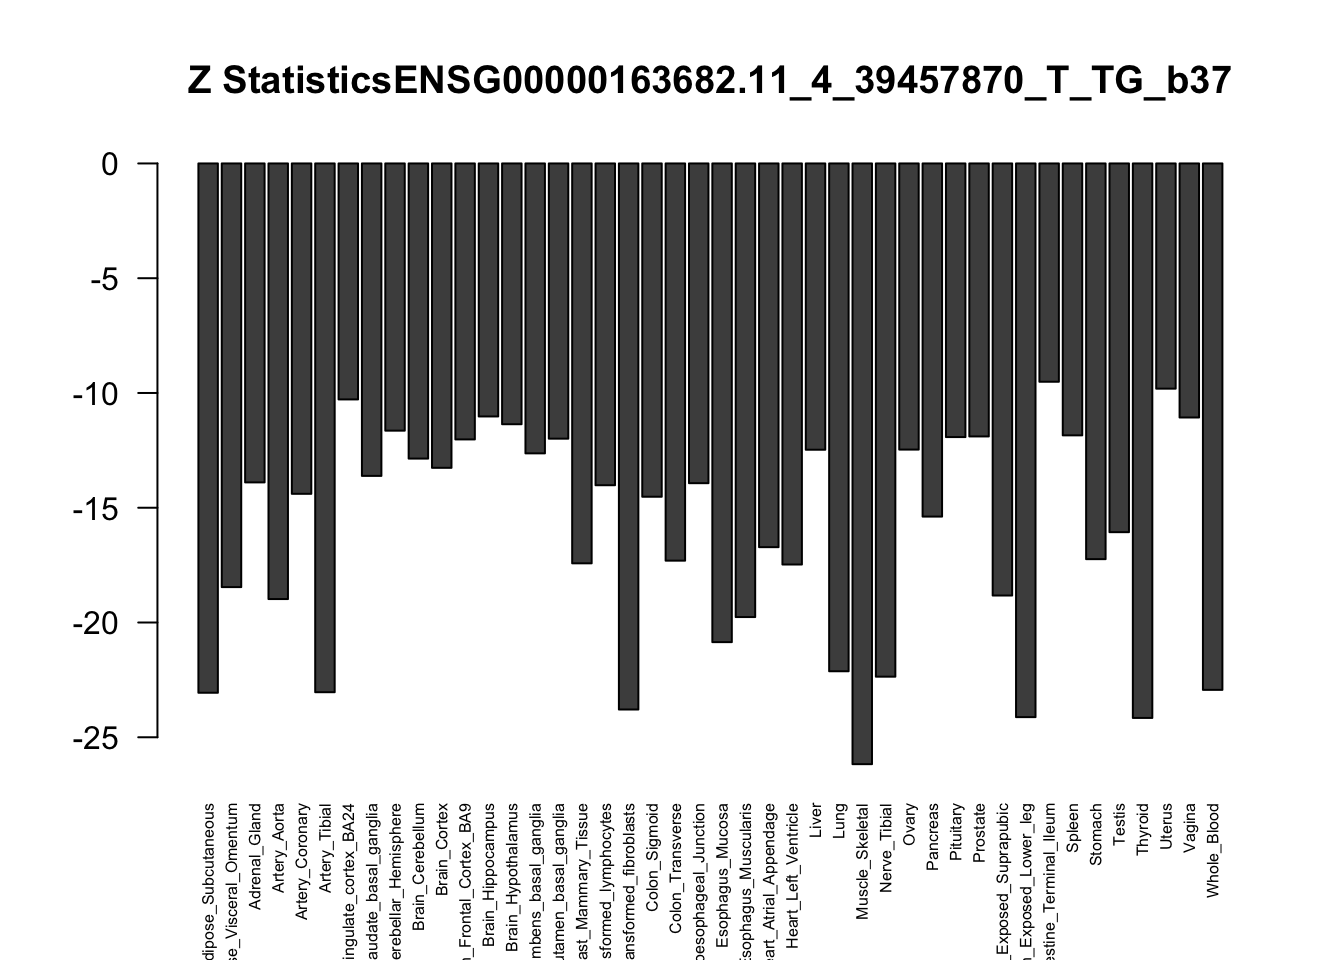
\includegraphics[width=5cm]{consistentz.png}
%\caption{An example in which consistency across tissues shrinks posteriors differently}
%\end{figure}
%
% \begin{figure}
%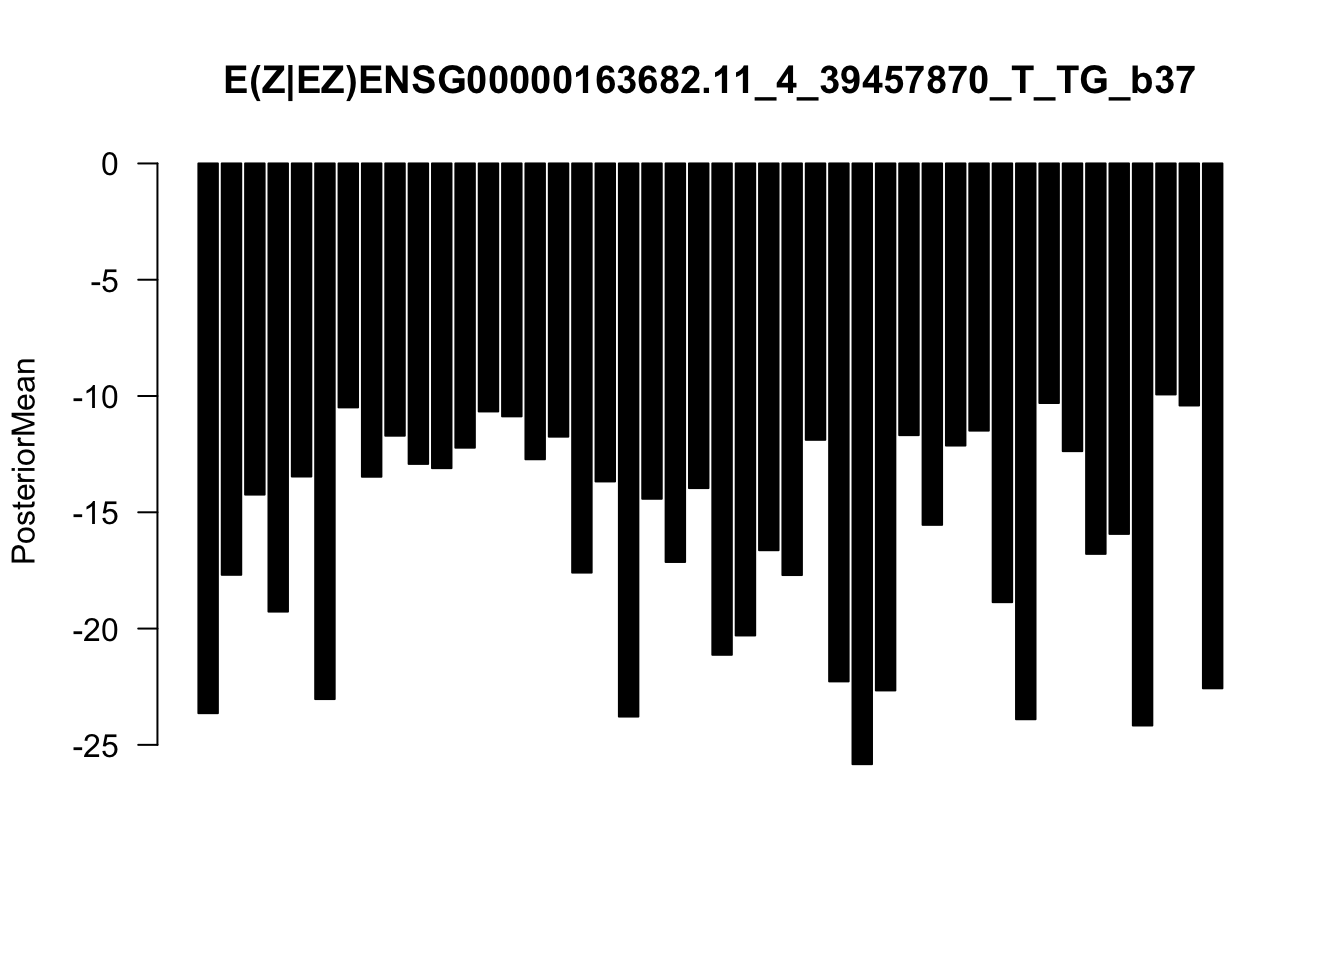
\includegraphics[width=5cm]{consistent.png}
%\caption{An example in which consistency across tissues shrinks posteriors differently}
%\end{figure}
%
% \begin{figure}
%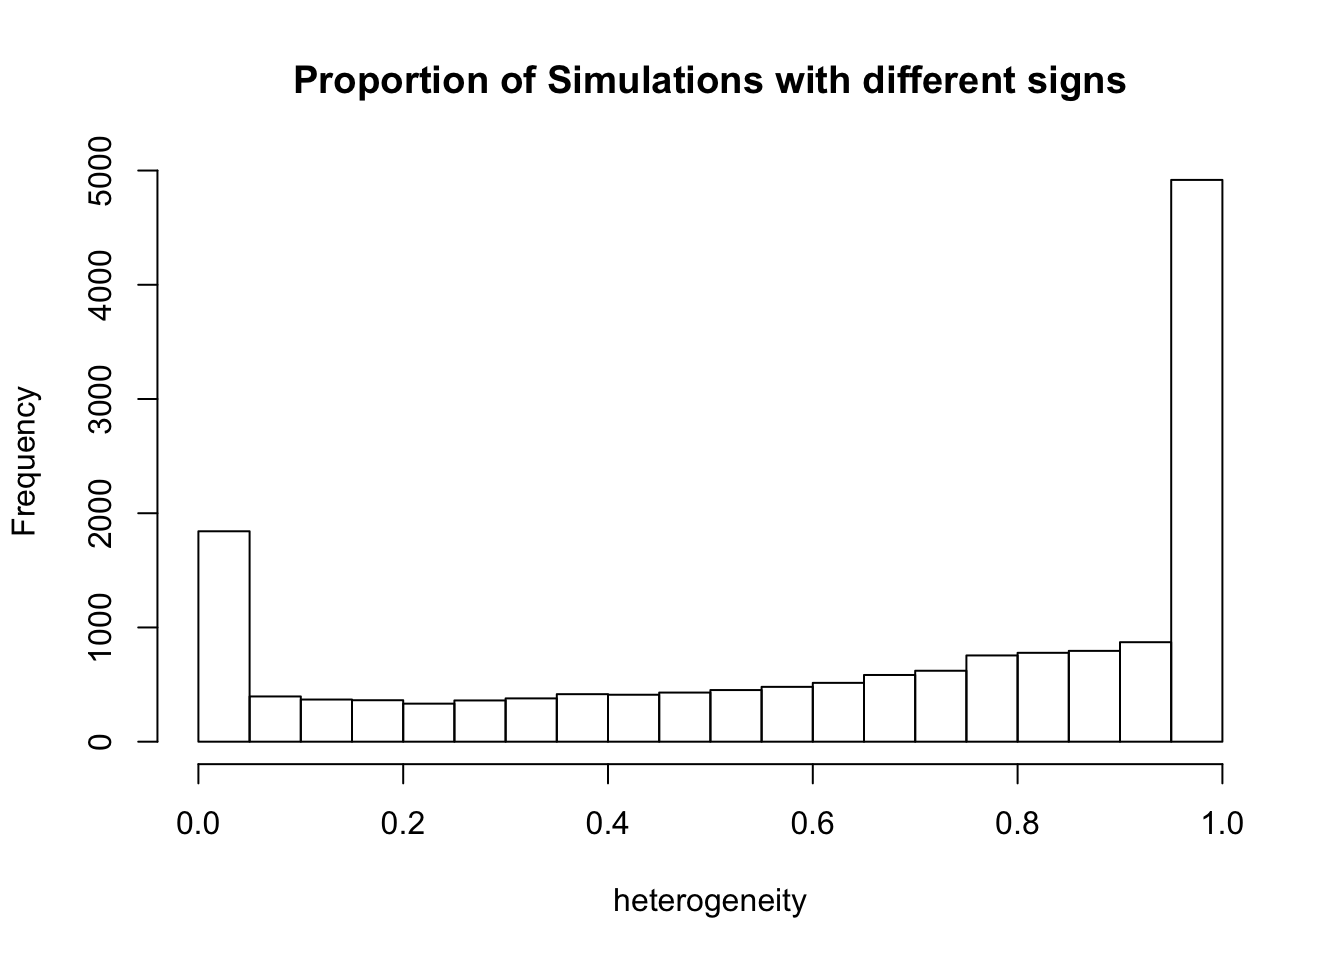
\includegraphics[width=5cm]{heterogeneity distribution-1.png}
%\caption{For each gene-snp pair, simulate 100 draws from mixture of multivariate normals, where the proportion of times in each component is determined by corresponding posterior weight $\tilde{pi_{kl}}$ We then count, for each gene-snp pair, the proportion of simulations that result in effects of a different sign in at least two tissues.}
%\end{figure}
%

\section*{Materials and Methods}


We assume the following mixture prior for the $R$ dimensional vector of true effects,  $\bm{b_{j}}$ represents the genetic effect of SNP-gene pair $j$ across $R$ = 44 tissues:

 \begin{equation}
  \bm{b_{j}} | \bm{\pi},\bf{U} \sim \sum_{k,l} \pi_{k,l} \;{\it N}_R(\bm{0}, \omega_l U_{k})
\end{equation}


%As mentioned above, 
Each component of the mixture distribution is characterized by these prior covariance matrices, $U_{k}$ which capture the pattern of effects across tissues. Critically, this prior distribution is the same for all $J$ - hence the hierarchical incorporation of shared information.

\subsection{ Covariance Matrices}

For a given $\omega_{l}$, we specify 4 `types' of $RxR$ prior covariance matrices $U_{k,l}$.
\begin{enumerate}

\item $U_{k=1,l}$ = $\omega_l$ $\mathbf{I}_{R}$

\item $U_{k=2,l}$ = $\omega_l$X_{z}$ The (naively) estimated tissue covariance matrix as estimated from the column-centered J \times R$ matrix of $Z$ statistics, $Z_{center}$: $\frac{1}{J}$ $Z_{center}$^{t}$ $Z_{center}$

\item $U_{k=3,l}$ = $\omega_l$ $\frac{1}{J}$ $V_{1...p}$ $d^{2}_{1...p}$   $V^{t}_{1..p}$ is the rank $p$ eigenvector approximation of the tissue covariance matrices, i.e., the sum of the first $p$ eigenvector approximations, where $\pcv_{1...p}$  represent the eigenvectors of the covariance matrix of tissues and $\pcd_{1...p}$ are the first $p$ eigenvalues.

\item $U_{k=4:4+Q-1,l}$ = $\frac{1}{J}(($\Lambda\mathbf{F})^{t} \Lambda \mathbf{F})_{q}$ corresponding to the $q_{th}$ sparse factor representation of the tissue covariance matrix %(not the sum of the first $q$, as above)

\item $U_{k=4+Q,l}$ = $\frac{1}{J}$ ($\($\Lambda \mathbf{F})^{t} \Lambda \mathbf{F}$ is the sparse factor representation of the tissue covariance matrix, estimated using all $q$ factors.



\item $U_{k=5+Q:R+4+Q,l}$ = $\frac{1}{J}$ $([1 0 0 . . ]'[1 0 0  . . .])$ %is the sparse factor representation of the tissue covariance matrix, estimated using all $q$ factors.
\item $U_{k=R+5+Q,l}$ = $\frac{1}{J}$ $([1 1 1 . . .]'[1 1 1 . . .])$
\item $[1 0 0 0 ...]$ or $[1 1 1  ...]$ represent configurations such that given membership,$\bm{b_{j}}$ arise from the same prior variance.
\end{itemize}



\subsection{Deconvolution}
To retrieve a `denoised' or `deconvoluted' estimate of the non-single rank dimensional reduction matrices, we then perform deconvolution after initializing the EM algorithm with  the matrices specified in (2), (3) and (5). The final results of this iterative procedure preserves the rank of the initialization matrix, and allows us to use the `true' effect component as missing data in deconvoluting the prior covariance matrices. In brief, this algorithm works by treating not only the component identity but also the true effect $\bm{{b}_{j}}$  as unobserved data, and maximizing the likelihood over the expectation of the complete data likelihood, considering the values $\bm{{b}_{j}}$ as extra missing data (in addition to the indicator variables $q_{ij}$) (Bovy et al, 2014). This allows us to write down the `full data' log likelihood as follows:

\begin{equation}

\begin{aligned}
\phi=\sum_{J} \sum_{K} q_{jk} ln \alpha_{k} \it{N}(\hat{\bm{{b}_{j}}}|0,U_{k}+V_{j})\\
\phi=\sum_{J} \sum_{K} q_{jk} ln \alpha_{k} \it{N}(\bm{{b}_{j}}|0,U_{k})


\end{aligned}
\end{equation}


Where $\alpha_{k}$ represents $\pi_k$ and $q_{jk}$ is the latent identifier variable.


%\subsection{Generation of List of Covariance Matrices}
%We then use these three non single-rank covariance matrix in place of our original choice of the empirical covariance matrix, SFA and SVD approximations. Here, I also used the Identity (K=1), 5 single-rank SFA factors (K=4-9), and the 44+1 $eqtlbma.lite$ configurations (K=10:54) in steps (7) and (8) to a assemble a full list of covariance matrices. Briefly, these  $eqtlbma.lite$ are an attempt to capture 'singleton' and 'fully shared' configurations in which the gene-snp pair is active in only one or all tissues. In the latter case, the variance of the distribution of underlying effect sizes is equal in all tissues.  This is 54 matrices, and we then proceed to chooses an $'L'$ element grid according to the range of effect sizes present in the initial 16,069 x 44 matrix of strong Z statistics to create a KxL list of covariance matrices. In the GTeX data set we choose a grid with 22 omegas for a total of 1188 covariance matrices.

\subsection{Posterior Quantities}
%Now that I have the estimated these prior mixture weights stored in the vector $\textbf{\pis}$. I proceed to the inference step, where I compute the posterior weights and corresponding posterior quantities across all original 16,069 gene-snp pairs. In brief, the posterior mean, post covariance matrix and tissue specific tail probabilities are computed across all K components for each gene snp pair, and then weighted according to the posterior weights. This is performed in the $\textbf{weightedquants}$ step.

We know that for a single multivariate {\it Normal}  the posterior on  $\bm{b} | U_0$ is  simply: 
\begin{equation}
\[
\bm{b} | \hat{\bm{b}} \sim {\it N}_R(\bm{\mu}_{1}, U_{1})
\]
\end{equation}
where:
\begin{itemize}
\item $\bm{\mu}_{1} = U_{1} (\hat{V}^{-1} \hat{\bm{b}})$;
\item $U_{1} = (U_{0}^{-1} + \hat{V}^{-1})^{-1}$.
\end{itemize}

Furthermore, a mixture-multivariate normal prior and a normal likelihood yields a mixture multivariate posterior, where the final posterior distribution is simply a weighted combination of multivariate normal distributions, each now characterized by it's posterior mean $\bm{\mu}_{1k}$ and covariance  $U_{1} = (U_{0}^{-1} + \hat{V}^{-1})^{-1}$.

\begin{equation}
\begin{aligned}
  \label{eq:mixpost}
p(\bm{b}_ | \hat{\bm{b}}, \hat{V}, \hat{\bm{\pi}} )
%&= \sum_{k=1,l=1}^{K,L} \sim {\it N}_R(\bm{\mu}_{1kl}, U_{1kl})%p(\bm{b}_{j} | \hat{\bm{b}}_{j}, \hat{V}_{j}, z_{j}=k,l) 
%p(z=k,l | \hat{\bm{b}}, \hat{V}, \hat{\bm{\pi} }),%v_{j}=1)
 %\\
= \sum_{k=1,l=1}^{K,L} \sim {\it N}_R(\bm{\mu}_{1kl}, U_{1kl})%,v_{j}=1) 
\tilde \pi_{k,l}

\end{aligned}
\end{equation}

where the posterior mixture weight $\tilde \pi_{k,l}$ is simply 

 
 \begin{equation}
 \label{post.pi}
\tilde \pi_{k,l} =\frac{ p(\hat{\bm{b}}_{j}| \hat{V}_{j}, z_{j}=k,l) \hat \pi_{kl}} {\sum_{k=1,l=1}^{K,L} p(\hat{\bm{b}}_{j}| \hat{V}_{j}, z_{j}=k,l) \hat\pi_{kl}}
\end{equation}


\section{Testing and Training}

In order to determine the optimal number and rank of the covariance matrices, we divide our data set into a training and test data set, each containing 8000 genes.

In the training set, we proceed as above: choosing the top SNP for each of the 8000 genes, creating a list of covariance matrices through deconvolution and grid selection of these top 'training gene-snp' pairs. 

Then, within the training data, we similarly choose a random set of gene-snp pairs (restricting our analysis to genes contained in the training set. Again, we choose 20,000 random-gene snp pairs and use the EM algorithm to learn the mixture proportions $\pi$  from this data set.

We then use the KxL vector of $\pi$ from the training set to estimate the log likelihood of each data point in the test data set. If our model is 'overfit' to the training data set, than a larger number of covariance matrices may actually decrease the test log-likelihood. 

I found that the K=1188 set of covariance matrices containing the Identity, the denoised empirical covariance matrix, rank 5 SFA approximation and rank 3 SVD approximation as well as 5 single-rank SFA factors and the 45 $eqtl.bma.lite$ configurations maximized this likelihood.




\section{Training and Testing Procedure: Estimating Hierarchical Weights}

We wish to choose the model which best maximizes the probability of observing the data set. 

Incomplete Data likelihood:
%Here, the total likelihood of the test data set over $K$ components: 

\begin{equation}
L(\bm\pi;{\hat{\bm{b}})} = \prod_{j=1}^J \sum_{k}^{K} \pi_{k} P(\hat{\bm{b_{j}}} | z_{j}=k)
\end{equation}

\begin{itemize}
\item  To estimate the hierarchical prior weights $\pi_{k}$: compute the likelihood at each each gene snp pair $j$ by evaluating the probability of observing $\bm{\hat{b}_{j}}$ given that we know the true $\bm{b_{j}}$ arises from component $k$
\item  Use the EM algorithm to estimate the optimal combination of weights: How often does this particular covariance matrix occur in the data?
\end{itemize}

We then use these weights to estimate the test set log likelihood.

% Results and Discussion can be combined.
\section*{Results}
%Nulla mi mi, venenatis sed ipsum varius, Table~\ref{table1} volutpat euismod diam. Proin rutrum vel massa non gravida. Quisque tempor sem et dignissim rutrum. Lorem ipsum dolor sit amet, consectetur adipiscing elit. Morbi at justo vitae nulla elementum commodo eu id massa. In vitae diam ac augue semper tincidunt eu ut eros. Fusce fringilla erat porttitor lectus cursus, vel sagittis arcu lobortis. Aliquam in enim semper, aliquam massa id, cursus neque. Praesent faucibus semper libero.
%
%
%\begin{table}[!ht]
%\begin{adjustwidth}{-2.25in}{0in} % Comment out/remove adjustwidth environment if table fits in text column.
%\caption{
%{\bf Table caption Nulla mi mi, venenatis sed ipsum varius, volutpat euismod diam.}}
%\begin{tabular}{|l|l|l|l|l|l|l|l|}
%\hline
%\multicolumn{4}{|l|}{\bf Heading1} & \multicolumn{4}{|l|}{\bf Heading2}\\ \hline
%$cell1 row1$ & cell2 row 1 & cell3 row 1 & cell4 row 1 & cell5 row 1 & cell6 row 1 & cell7 row 1 & cell8 row 1\\ \hline
%$cell1 row2$ & cell2 row 2 & cell3 row 2 & cell4 row 2 & cell5 row 2 & cell6 row 2 & cell7 row 2 & cell8 row 2\\ \hline
%$cell1 row3$ & cell2 row 3 & cell3 row 3 & cell4 row 3 & cell5 row 3 & cell6 row 3 & cell7 row 3 & cell8 row 3\\ \hline
%\end{tabular}
%\begin{flushleft} Table notes Phasellus venenatis, tortor nec vestibulum mattis, massa tortor interdum felis, nec pellentesque metus tortor nec nisl. Ut ornare mauris tellus, vel dapibus arcu suscipit sed.
%\end{flushleft}
%\label{table1}
%\end{adjustwidth}
%\end{table}
%
%
%
%\subsection*{\lorem\ and \ipsum\ Nunc blandit a tortor.}
%
%Maecenas convallis mauris sit amet sem ultrices gravida. Etiam eget sapien nibh. Sed ac ipsum eget enim egestas ullamcorper nec euismod ligula. Curabitur fringilla pulvinar lectus consectetur pellentesque. Quisque augue sem, tincidunt sit amet feugiat eget, ullamcorper sed velit. Sed non aliquet felis. Lorem ipsum dolor sit amet, consectetur adipiscing elit. Mauris commodo justo ac dui pretium imperdiet. Sed suscipit iaculis mi at feugiat. 
%
%\subsection*{Sed ac quam id nisi malesuada congue.}
%
%Nulla mi mi, venenatis sed ipsum varius, volutpat euismod diam. Proin rutrum vel massa non gravida. Quisque tempor sem et dignissim rutrum. Lorem ipsum dolor sit amet, consectetur adipiscing elit. Morbi at justo vitae nulla elementum commodo eu id massa. In vitae diam ac augue semper tincidunt eu ut eros. Fusce fringilla erat porttitor lectus cursus, vel sagittis arcu lobortis. Aliquam in enim semper, aliquam massa id, cursus neque. Praesent faucibus semper libero.
%
%% Please do not create a heading level below \subsection. For 3rd level headings, use \paragraph{}. 
%\subsection*{Subsection 1}
%Nulla mi mi, venenatis sed ipsum varius, volutpat euismod diam. Proin rutrum vel massa non gravida. Quisque tempor sem et dignissim rutrum. Lorem ipsum dolor sit amet, consectetur adipiscing elit. Morbi at justo vitae nulla elementum commodo eu id massa. In vitae diam ac augue semper tincidunt eu ut eros. Fusce fringilla erat porttitor lectus cursus, vel sagittis arcu lobortis. Aliquam in enim semper, aliquam massa id, cursus neque. Praesent faucibus semper libero.
%
%\subsection*{Subsection 2}
%\paragraph{3rd Level Heading.} Nulla mi mi, venenatis sed ipsum varius, volutpat euismod diam. Proin rutrum vel massa non gravida. Quisque tempor sem et dignissim rutrum. Lorem ipsum dolor sit amet, consectetur adipiscing elit. Morbi at justo vitae nulla elementum commodo eu id massa. In vitae diam ac augue semper tincidunt eu ut eros. Fusce fringilla erat porttitor lectus cursus, vel sagittis arcu lobortis. Aliquam in enim semper, aliquam massa id, cursus neque. Praesent faucibus semper libero.

\section*{Discussion}
%Nulla mi mi, venenatis sed ipsum varius, Table~\ref{table1} volutpat euismod diam. Proin rutrum vel massa non gravida. Quisque tempor sem et dignissim rutrum. Lorem ipsum dolor sit amet, consectetur adipiscing elit. Morbi at justo vitae nulla elementum commodo eu id massa. In vitae diam ac augue semper tincidunt eu ut eros. Fusce fringilla erat porttitor lectus cursus, vel sagittis arcu lobortis. Aliquam in enim semper, aliquam massa id, cursus neque. Praesent faucibus semper libero.
%
%\subsection*{\lorem\ and \ipsum\ Nunc blandit a tortor.}
%
%CO\textsubscript{2} Maecenas convallis mauris sit amet sem ultrices gravida. Etiam eget sapien nibh. Sed ac ipsum eget enim egestas ullamcorper nec euismod ligula. Curabitur fringilla pulvinar lectus consectetur pellentesque. Quisque augue sem, tincidunt sit amet feugiat eget, ullamcorper sed velit. 
%
%Sed non aliquet felis. Lorem ipsum dolor sit amet, consectetur adipiscing elit. Mauris commodo justo ac dui pretium imperdiet. Sed suscipit iaculis mi at feugiat. Ut neque ipsum, luctus id lacus ut, laoreet scelerisque urna. Phasellus venenatis, tortor nec vestibulum mattis, massa tortor interdum felis, nec pellentesque metus tortor nec nisl. Ut ornare mauris tellus, vel dapibus arcu suscipit sed. Nam condimentum sem eget mollis euismod. Nullam dui urna, gravida venenatis dui et, tincidunt sodales ex. Nunc est dui, sodales sed mauris nec, auctor sagittis leo. Aliquam tincidunt, ex in facilisis elementum, libero lectus luctus est, non vulputate nisl augue at dolor. For more information, see \nameref{S1_Text}.
%
\section*{Supporting Information}

% Include only the SI item label in the subsection heading. Use the \nameref{label} command to cite SI items in the text.
%\subsection*{S1 Video}
%\label{S1_Video}
%{\bf Bold the first sentence.}  Maecenas convallis mauris sit amet sem ultrices gravida. Etiam eget sapien nibh. Sed ac ipsum eget enim egestas ullamcorper nec euismod ligula. Curabitur fringilla pulvinar lectus consectetur pellentesque.
%
%\subsection*{S1 Text}
%\label{S1_Text}
%{\bf Lorem Ipsum.} Maecenas convallis mauris sit amet sem ultrices gravida. Etiam eget sapien nibh. Sed ac ipsum eget enim egestas ullamcorper nec euismod ligula. Curabitur fringilla pulvinar lectus consectetur pellentesque.
%
%\subsection*{S1 Fig}
%\label{S1_Fig}
%{\bf Lorem Ipsum.} Maecenas convallis mauris sit amet sem ultrices gravida. Etiam eget sapien nibh. Sed ac ipsum eget enim egestas ullamcorper nec euismod ligula. Curabitur fringilla pulvinar lectus consectetur pellentesque.
%
%\subsection*{S2 Fig}
%\label{S2_Fig}
%{\bf Lorem Ipsum.} Maecenas convallis mauris sit amet sem ultrices gravida. Etiam eget sapien nibh. Sed ac ipsum eget enim egestas ullamcorper nec euismod ligula. Curabitur fringilla pulvinar lectus consectetur pellentesque.
%
%\subsection*{S1 Table}
%\label{S1_Table}
%{\bf Lorem Ipsum.} Maecenas convallis mauris sit amet sem ultrices gravida. Etiam eget sapien nibh. Sed ac ipsum eget enim egestas ullamcorper nec euismod ligula. Curabitur fringilla pulvinar lectus consectetur pellentesque.
%
\section*{Acknowledgments}
%Cras egestas velit mauris, eu mollis turpis pellentesque sit amet. Interdum et malesuada fames ac ante ipsum primis in faucibus. Nam id pretium nisi. Sed ac quam id nisi malesuada congue. Sed interdum aliquet augue, at pellentesque quam rhoncus vitae.

\nolinenumbers

%\section*{References}
% Either type in your references using
% \begin{thebibliography}{}
% \bibitem{}
% Text
% \end{thebibliography}
%
% OR
%
% Compile your BiBTeX database using our plos2015.bst
% style file and paste the contents of your .bbl file
% here.
% 
\begin{thebibliography}{10}
\bibitem{bib1}
Devaraju P, Gulati R, Antony PT, Mithun CB, Negi VS. Susceptibility to SLE in South Indian Tamils may be influenced by genetic selection pressure on TLR2 and TLR9 genes. Mol Immunol. 2014 Nov 22. pii: S0161-5890(14)00313-7. doi: 10.1016/j.molimm.2014.11.005

\bibitem{bib2}
Huynen MMTE, Martens P, Hilderlink HBM. The health impacts of globalisation: a conceptual framework. Global Health. 2005;1: 14. Available: http://www.globalizationandhealth.com/content/1/1/14.

\end{thebibliography}



\end{document}

